\section{Architecture on Google cloud} \label{sec:google}

As the RSP services were built for cloud deployment (see \autoref{sec:deploy}), they are elastically scalable and easy to set up.
The Portal and Notebook Aspects each run as an application (in the ArgoCD sense), while each API within the API Aspect is its own application.
They rely on a common authentication and authorization (and throttling) infrastructure to ensure that only science users with appropriate data rights have access.

The back-end communication with the USDF services hosting the bulk of the data products is mediated through two primary interfaces: a relational database query interface for catalogs that can talk to the scalable, distributed Qserv service and the client/server Butler for access to image and other file-based data products.

The client/server Butler manages metadata about data products and user rights to access those products.
It can generate signed URLs that provide anonymous, bearer access for a limited time to specific files in the underlying storage at the USDF.
These URLs can be consumed by RSP services, or they can be returned directly to science users, avoiding mediation of network traffic by Google (which would count as egress).
The client/server Butler is further discussed in this SPIE paper \cite{2024SPIE13101.129Jtmp}.
For performance reasons, we may host a subset of the data products, either statically or dynamically chosen (or a combination of both), in the cloud.

We also will provide a service for advanced science users to execute batch jobs.
Since these jobs are expected to involve processing a large amount of data, it makes sense to run them at the USDF.
We can either have these specialized users obtain SLAC accounts, or we can use batch processing tools designed for the grid to manage the jobs and corresponding resource and access controls.

We reported on the Interim Data Facility (IDF) already at ADASS\cite{2021arXiv211115030O}.
Our services have been operating on Google Cloud for over three years now.
In Data Preview 0.3 on IDF, the Qserv database instance was moved to SLAC, so we have demonstrated this also works.


\begin{figure}
\begin{centering}
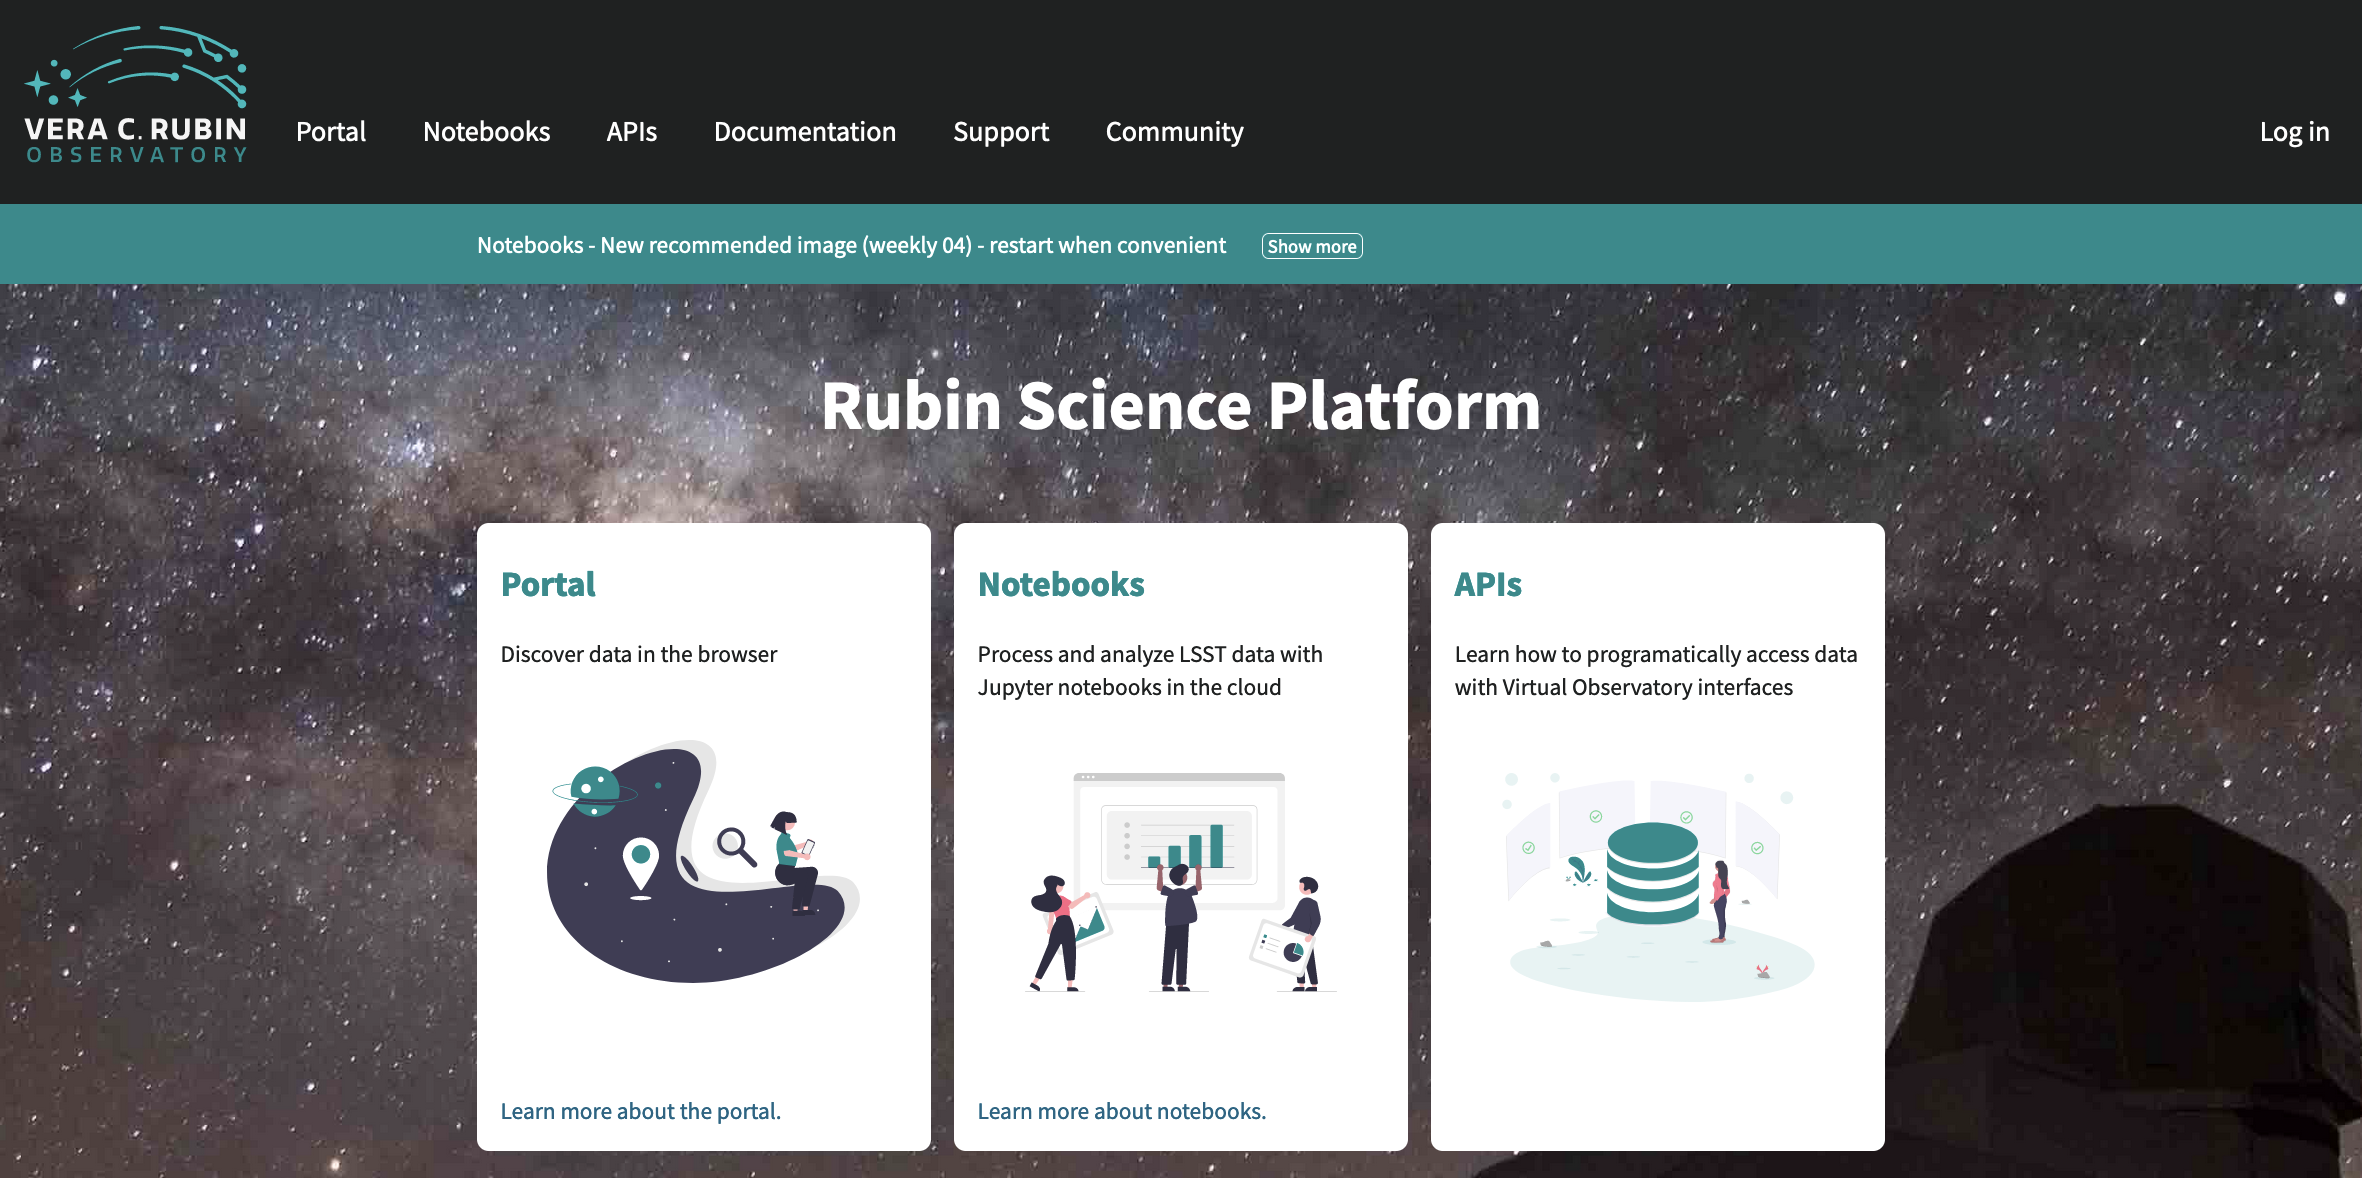
\includegraphics[width=0.9\textwidth]{RSP.png}
	\caption{ Users hosted on Google will typically use the Rubin Science Platform (RSP) depicted here.  \label{fig:rsp}}
\end{centering}
\end{figure}
